\lab{Application}{Facial Recognition using Eigenfaces}{Facial Recognition using Eigenfaces}
\label{lab:FacialRecognition}

\objective{In this lab we use the singular value decomposition to build a facial recognition system.}

Suppose we have a large database containing images of human faces together with identification information for each face.
Given an unidentified facial image, we would like to find a matching face in the database, thereby identifying the person in the image.
Such a task is known as \emph{facial recognition}.
This task may come up, for example, in law enforcement, when attempting to identify unknown persons in surveillance footage.
As humans, it is generally easy to compare two face images and determine whether the faces belong to the same person.
However, it becomes impractical for humans to visually compare one face image with several thousand other face images in a database.
Hence, we need a computational technique that automates the process of facial recognition.
One particularly simple and effective technique is known as \emph{eigenfaces}, which we now explore.

\section*{Eigenfaces}
The method of eigenfaces provides a mathematical and computational technique for efficiently storing and querying a database of face images.
As the name suggests, this method involves eigenvalues and eigenvectors of matrices related to the collection of face images at hand.
At its core, the method of eigenfaces maps each face image to a low-dimensional representation in a way that highlights the distinguishing
characteristics of the face while suppressing the irrelevant and unnecessary details.
In this light, eigenfaces can be viewed as a means of dimensionality reduction.
Let's get into the nuts and bolts of how this works.

Suppose we have a collection of $k$ face images represented as vectors $f_1, f_2, \ldots, f_k$ of length $l$.
(A digital image is normally represented by a $m \times n$ array of pixel values, but we can represented as a vector in $\mathbb{R}^{mn}$ by simply concatenating the rows of the array.)
Define the \emph{mean face} $\mu$ to be the average of each face vector:
\[
\mu = \frac{1}{k}\sum_{i=1}^k f_i.
\]
\begin{figure}
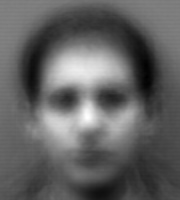
\includegraphics[width=0.3\textwidth]{meanFace.png}
\caption{The mean face.}
\label{facialRecognition:meanFace}
\end{figure}



\begin{problem}
\label{prob:getTrainingFaces}
Download the \li{faces94} face image database found at \url{http://cswww.essex.ac.uk/mv/allfaces/faces94.html} and extract the files.
You should now have a directory named ``faces94", which contains multiple face images each of a large collection of individuals.
We will construct a database of face images by selecting exactly one face image for each person in the directory.
Execute the following code to construct the collection of faces (you may need to change the variable \li{path} to point to the location
of the \li{faces94} directory on your machine):
\begin{lstlisting}
>>> import numpy as np
>>> from os import walk
>>> from scipy.ndimage import imread
>>> # these are the dimensions of the images
>>> w = 200
>>> h = 180
>>> # traverse the directory, get one image per subdirectory
>>> path = "./faces94"
>>> faces = []
>>> for (dirpath, dirnames, filenames) in walk(path):
>>>     for f in filenames:
>>>         if f[-3:]=="jpg": # only get jpg images
>>>             # load image, convert to grayscale, flatten into vector
>>>             face = imread(dirpath+"/"+f).mean(axis=2).ravel()
>>>             faces.append(face)
>>>             break
>>> # put all the face vectors column-wise into a matrix
>>> F = np.array(faces).T
\end{lstlisting}
The array \li{F} should be a $360000 \times 153$ matrix whose columns consist of 153 face images.
\end{problem}
\begin{problem}
\label{prob:meanFace}
Calculate the mean face image \li{mu} from the face image array \li{F} that you obtained in problem \ref{prob:getTrainingFaces}.
This can be done easily using \li{np.mean} and specifying the correct axis.

Plot the mean face.
As a convenience, you may use the following function to plot the image given just the flat vector representation:
\begin{lstlisting}
>>> from matplotlib import pyplot as plt
>>> import matplotlib.cm as cm
>>> def show(im, w=200, h=180):
>>>     """
>>>     Plot the w by h image whose pixel values are given by the array im.
>>>     """
>>>     plt.imshow(im.reshape((w,h)), cmap=cm.Greys_r)
>>>     plt.show()
>>> # given that you have calculated the mean face mu, show it
>>> show(mu)
\end{lstlisting}
Your mean face should match that shown in Figure \ref{facialRecognition:meanFace}.
\end{problem}
\begin{figure}
\begin{subfigure}[b]{0.3\textwidth}
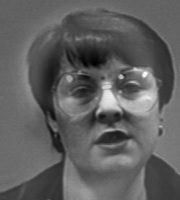
\includegraphics[width=\textwidth]{differenceFace0.png}
\end{subfigure}
\begin{subfigure}[b]{0.3\textwidth}
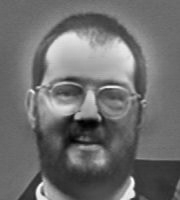
\includegraphics[width=\textwidth]{differenceFace1.png}
\end{subfigure}
\begin{subfigure}[b]{0.3\textwidth}
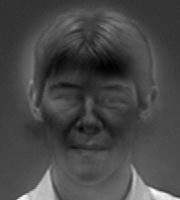
\includegraphics[width=\textwidth]{differenceFace2.png}
\end{subfigure}
\caption{Three mean-shifted faces from the dataset.}
\label{facialRecognition:differenceFaces}
\end{figure}
For each $i = 1,\ldots, k$, define $\bar{f}_i := f_i - \mu$.
The mean-shifted face vector $\bar{f}_i$ represents how the $i$-th face deviates from the average, and thus captures more directly the unique and distinguishing features of the face.
Now form the $l \times K$ matrix $A$ whose columns are given by the mean-shifted face vectors, i.e.
\[
A = \begin{bmatrix}
\bar{f}_1 & \bar{f}_2 & \cdots & \bar{f}_k
\end{bmatrix}.
\]
\begin{problem}
Using the face matrix \li{F} and the mean face \li{mu} from problems \ref{prob:getTrainingFaces} and \ref{prob:meanFace}, calculate the
matrix of mean-shifted face vectors \li{A}.
(This can be done in a nice, vectorized manner using array broadcasting.)
Plot the first mean-shifted face, i.e. the first column of the matrix \li{A}.
It should match the first face in Figure \ref{facialRecognition:differenceFaces}.
\end{problem}

Thus far, we have obtained the mean face vector $\mu$ and a representation of our collection of face images via the matrix $A$.
With just this matrix and the mean vector, how might we go about searching our collection of face images for the closest match to a new face image $g$?
A straightforward approach is to subtract the mean face vector from $g$, obtaining $\bar{g} = g-\mu$, and then compute the Euclidean distance from
$\bar{g}$ to each mean-shifted face vector $\bar{f}_i$, i.e. compute the Euclidean distance between $\bar{g}$ and each column of $A$.
Having done so, we can then choose the index $i$ where this distance $\|\bar{g}-\bar{f}_i\|_2$ is smallest, and return the $i$-th face image as the best match.
Although this approach is quite sensible, it become computationally expensive as the number and size of our face images increases.
What we need, then, is a way to reduce the dimensionality of our images.

\begin{comment}
The discussion in the paragraph below needs some work.
I need to better understand why the eigenfaces basis works so well.

Although this approach is quite sensible, there are a few issues.
Firstly, as the number of face images in our database grows large, both storing the full matrix $A$ and computing $\|\bar{g}-\bar{f}_i\|_2$ for all $i$
become increasingly difficult from a computational standpoint.
Secondly -- and this is the more important point -- calculating the Euclidean distance between two face images in the standard basis may not be the best measure
of how similar the two faces are (and empirical evidence supports this).
For example, if we have two images of the same face but with different backgrounds, the Euclidean distance between the face vectors may be very large,
since in the standard basis, every pixel is weighted equally.
Given these issues, it is natural to ask ourselves whether there exists a low-dimensional subspace with a basis in which we can represent our
face images with minimal error and where the Euclidean distance is a more robust measure of face similarity.
\end{comment}

Since the face images all have much in common, we have reason to hope that they all lie (nearly) in a low-dimensional subspace of $\mathbb{R}^l$.
The singular value decomposition of $A$ gives us just such a subspace.
In particular, if we write the singular value decomposition as
\[
A = U\Sigma V^H,
\]
then the columns of $U$ corresponding to the positive singular values form an orthonormal basis for the columns of $A$.
Recall that there are $r$ positive singular values, where $r$ is the rank of $A$.
Hence, if $r \ll l$, then we have found a low-dimensional subspace in which to represent our face vectors.
We call this subspace the \emph{eigenface subspace}, and we call each basis vector (i.e. each column of $U$ corresponding
to a positive singular value) an \emph{eigenface}.
\begin{figure}
\begin{subfigure}[b]{0.3\textwidth}
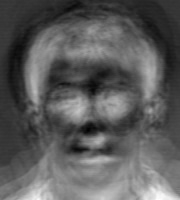
\includegraphics[width=\textwidth]{eigenface0.png}
\end{subfigure}
\begin{subfigure}[b]{0.3\textwidth}
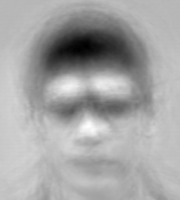
\includegraphics[width=\textwidth]{eigenface1.png}
\end{subfigure}
\begin{subfigure}[b]{0.3\textwidth}
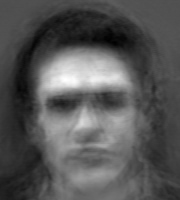
\includegraphics[width=\textwidth]{eigenface2.png}
\end{subfigure}
\caption{The top three eigenfaces.}
\label{facialRecognition:eigenfaces}
\end{figure}
\begin{problem}
\label{prob:svd}
Calculate the singular value decomposition of the matrix \li{A} as follows:
\begin{lstlisting}
>>> from scipy imort linalg as la
>>> U,Sig,Vh = la.svd(A, full_matrices=False)
\end{lstlisting}
The keyword argument \li{full_matrices=False} cause the function to only return the columns of $U$ and $V$ corresponding
to positive singular values. Hence, \li{U} should be a $36000\times 153$ matrix whose columns are the eigenfaces.
Plot the first eigenface (i.e. the first column of \li{U}).
It should match the first eigenface shown in Figure \ref{facialRecognition:eigenfaces}.
By plotting some of the other eigenfaces, note that each has face-like properties, and different eigenfaces tend to capture different
types of facial structures.
\end{problem}

Not all of the eigenfaces are equally important, however.
In particular, the eigenfaces corresponding to the singular values closest to 0 contribute the least, on average, to the face vectors in $A$.
Thus, we can get away with only using the eigenfaces corresponding to the $n$ largest singular values (call these the top $n$ eigenfaces).
This is important when the rank $r$ is still too large to be practical.
Define $U_n$ to be the $l \times n$ matrix whose columns consist of the top $n$ eigenfaces.
The the coordinate vector of $\bar{f}_i$ in terms of these top $n$ eigenfaces is given by
\[
\hat{f}_i := U_n^H\bar{f}_i.
\]
Hence the matrix $\hat{A}$ defined by
\[
\hat{A}_n = \begin{bmatrix}
\hat{f}_1 & \hat{f}_2 & \ldots & \hat{f}_k
\end{bmatrix}
= U_n^HA
\]
contains as its columns the coordinate vectors of the face images in the top $n$ eigenfaces basis.
Note that $\hat{A}$ is an $n \times k$ matrix, and is therefore much smaller than the original $l \times k$ matrix $A$.
\begin{problem}
\label{prob:top_n}
The columns of the matrix \li{U} that you computed in problem \ref{prob:svd} are already ordered according to descending singular values.
Thus, the first $n$ columns of \li{U} give the top $n$ eigenfaces.
Write a function \li{nEigenfaces} that takes as input \li{U}, \li{A}, and an integer $n$, and returns the matrices $U_n$ and $\hat{A}_n$ as described above.
\end{problem}
\begin{figure}
\begin{subfigure}[b]{0.3\textwidth}
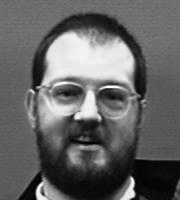
\includegraphics[width=\textwidth]{rebuiltAll.png}
\caption{All of the eigenfaces.}
\end{subfigure}
\begin{subfigure}[b]{0.3\textwidth}
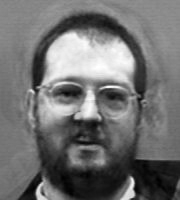
\includegraphics[width=\textwidth]{rebuiltHalf.png}
\caption{1/2 of the eigenfaces.}
\end{subfigure}
\begin{subfigure}[b]{0.3\textwidth}
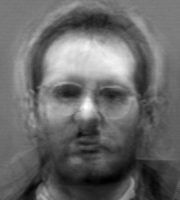
\includegraphics[width=\textwidth]{rebuiltFourth.png}
\caption{1/4 of the eigenfaces.}
\end{subfigure}
\caption{Image rebuilt with varying number of eigenfaces}
\label{facialRecognition:rebuiltImage}
\end{figure}
Of course, moving to a lower-dimensional subspace by using only the top $n$ eigenfaces introduces some error, in the sense that we cannot perfectly
reconstruct the face images from their coordinate vectors.
However, this error is tolerable, provided $n$ is not \emph{too} small.
Note that we can approximately reconstruct $\bar{f}_i$ from the coordinate vector $\hat{f}_i$ by
\[
\bar{f}_i \approx U_n\hat{f}_i.
\]
See Figure \ref{facialRecognition:rebuiltImage} for examples of reconstructed face images giving different numbers of eigenfaces.

We now have a low-dimensional representation of our database of face images given by $\hat{A}_n$, an array of eigenfaces given by $U_n$,
and the mean face $\mu$. Using just these objects, we can now perform facial recognition.
Let $g$ be a face vector.
We seek to find the face vector $f_i$ in the database that is closest to $g$.
In order to do so, we must process $g$ just as we processed each $f_i$, namely by subtracting out the mean face and then projecting onto the
eigenfaces basis.
Doing so yields the low-dimensional representation $\hat{g}$, given by
\[
\hat{g} = U_n^H(g-\mu).
\]
We then return the matching face image $f_{i^*}$, where
\[
i^* = \text{argmin}_i \|\hat{f}_i - \hat{g}\|_2.
\]
\begin{problem}
\label{prob:nearest}
Write a function \li{findNearest} that accepts a matrix $M$ of shape $a \times b$ and a vector $x$
of length $a$, and returns the index of the column of $M$ that is closest to $x$ with respect to Euclidean distance.
Using the NumPy functions \li{np.linalg.norm} and \li{np.argmin} will be useful here.
\end{problem}

\begin{problem}
\label{prob:match}
We will perform facial recognition on additional images from the \li{faces94} dataset.


Use the following code to build an array of additional images from the dataset:
\begin{lstlisting}
>>> # let's gather some random images from the directory, and try to recognize them!
>>> n_tests = 10
>>> test_files = []
>>> for (dirpath, dirnames, filenames) in walk(path):
>>>     for f in filenames:
>>>         if f[-3:]=="jpg": # only get jpg images
>>>             test_files.append(dirpath+"/"+f)
>>> test_files = sample(test_files, n_tests)
>>> test_images = np.array([imread(f).mean(axis=2).ravel() for f in test_files]).T
\end{lstlisting}
You can change the variable \li{n_tests} to increase or decrease the number of face images to test.

Using your function \li{findNearest} from problem \ref{prob:nearest}, loop through the test images and find
the index of best matching image from the database.
As you do so, plot the test face alongside the matching face from the database to determine whether your system
really is properly recognizing the faces.
Use the following code to conveniently plot two face vectors side-by-side:
\begin{lstlisting}
>>> def show2(im1, im2, w=200, h=180):
>>>     """Plot face vectors im1 and im2 side-by-side."""
>>>     plt.subplot(121)
>>>     plt.imshow(im1.reshape((w,h)), cmap=cm.Greys_r)
>>>     plt.subplot(122)
>>>     plt.imshow(im2.reshape((w,h)), cmap=cm.Greys_r)
>>>     plt.show()
\end{lstlisting}

Repeat this experiment for different values of $n$, the number of eigenfaces to include.
The system should improve as $n$ gets larger.
\end{problem}

By this point, you have created a basic facial recognition system.
We can extend the system to detect when a face doesn't match anything currently in the database, and then add this new face into the database.
We can also make the system more robust by including multiple pictures of the same face with different expressions and lighting conditions.
Although there are other approaches to facial recognition that utilize more complex techniques, the method of eigenfaces remains
a wonderfully simple and effective solution and provides another illustration of the usefulness of the singular value decomposition in a variety of applications.

\begin{comment}
What remains is some old content.

\section*{Preparing the data}

Through the course of this lab we will be building a class called \li{FacialRec} to handle everything in the facial recognition system.
In the \li{specs.py} file included with this lab there is an outline of this class along with some helper functions to help us test our system.

To populate our database, we will need some images of faces.
There are many databases available online, many of which would work with our project.
However, the algorithm which we will use is not completely robust, it requires the images to have similar lighting conditions and head positions.
Tilted head, dark lighting, wearing glasses, and different hairstyles can disrupt the algorithm.
Therefore, we need a database that contains images with consistent lighting and head posistions.
Also, to make the programming easier, we would like the images to be of the same file type and size.
The University of Essex has such a database at http://cswww.essex.ac.uk/mv/allfaces/index.html, (as well as other databases with varied head positions and lighting conditions) which we will use.

The function \li{getImages} included in the specifications file loads all the JPG files from a directory into a 3 dimensional array.
The first dimension specifices the image while the other two give the grayscale image in a 2D array.
We can also use the function \li{showImage} to display the 2D grayscale images.
This will be useful for testing the database.

\begin{problem}
Download the faces94 database from the University of Essex from http://cswww.essex.ac.uk/mv/allfaces/index.html.
Initialize a \li{FacialRec} object using the file path to the directory and have it use every 50$^{th}$ face in the database.
Also, for testing purposes, use the function \li{getImages} to put the whole database into an array of images.
Then use \li{showImage} to show the first image.
\end{problem}

Now that we have images, we need to calculate a few things before we can compute the eigenfaces from the covariance matrix.
We have already reduced the images to grayscale images in \li{getImages} to make computations easier.
Now we need the mean face of all the faces in the database. The mean face is a 2D array of each pixel average across the database.
Next we need to zero out the images using the mean face.
We will substract the mean face from each face in the database, giving the the difference faces.
Then we flatten the each 2D image into a one dimensional vector so that we have each image described in single vector space.

\begin{problem}
Implement the functions \li{initMeanImage} and \li{initDifferences}.
\li{initMeanImage} should store in \li{self.meanImage} the image of the means across each pixel in the entire database.
\li{initDifferences} should first initilize \li{self.differenceFaces} to be an array of each image in the database minus the mean image.
\li{self.differenceVectors} should be the matrix with the flattened vector of each image in the database as its rows.
If the database has 75 images each of size $200 \times 180$, then \li{self.differenceVectors} should be $75 \times 36000$.
Also, plot the mean face and the first difference face.
\end{problem}


\section*{Computing the Eigenfaces with SVD}

With these pelimanaries ready, we are now able to construct the Eigenfaces of the system from the covariance matrix.
At this point we have each image descibed in a vector space with as many pixels as there are in each image.
With the database we are using, this is a 36000 dimensional vector space.
There are too many random variables to work with at this point to work with, so we need to find some way to simplify the vector space.

We do this using the eigenvectors of the covariance matrix (which we call the eigenfaces).
The eigenfaces form a basis of all possible faces, so all faces could be expressed as a linear combination of eigenfaces from the covariance matrix gathered from faces in the database.
The corresponding eigenvalues of the eigenfaces give the weight or importance of each eigenface.
Now there the covariance matrix is still very large 36000 and could have many distinct eigenvectors.
However, only eigenfaces corresponding to higher eigenvalues really make a difference.
Infact, it turns out that there are only as many eigenvalues as there are images in the database.

Recall that taking the SVD of a real valued matrix $A$ gives us the eigenvectors of the matrix $AA^T$ in the columns of $V$.
If the difference vectors are denoted by $E$, then the covariance matrix is $C = EE^T$.
It then follows that we can use the SVD of $E$ to compute the eigenvectors of $C = EE^T$.

The \li{svd} function from \li{scipy.linalg} returns $U,V,V^T$. You can then get the eigenfaces with a call like
\begin{lstlisting}
u,s,vT = la.svd(self.differenceVectors,full_matricies=False)
self.eigenfaces = vT
\end{lstlisting}
This will put into \li{eigenfaces} the eigenfaces of the database as its rows.

\begin{problem}
Implement the function \li{initEigenfaces} by computing the eigenfaces of the images in the database using the SVD and storing them in \li{self.eigenfaces}.
The eigenfaces should be in the columns of \li{self.eigenfaces} so that it becomes a $36000 \times 75$ matrix.
Plot the first three eigenfaces.
\end{problem}



With the eigenfaces computed, we can now convert vectors representing faces into the eigenface space and back.
To convert to the eigenface space we first subtract off the mean face, flatten the vector, then project the vector on the eigenfaces.
To rebuild an image from its representation in eigenfaces, we simply add up the linear combination of eigenfaces then add back in the mean.

\begin{problem}
Implement the functions \li{projectToImageFaceSpace} and \li{rebuildFromEigenfaces}.
\li{projectToImageFaceSpace} should project an image into its coordinates in the basis of the eigenfaces.
\li{rebuildFromEigenfaces} should undo that projection by taking the coordinates in the eigenface space, projecting them back, and reshaping the image.
\end{problem}



\section*{Creating the Facial Recognition System}

The facial recognition database is almost done.
Given a face to seach for, we only have to project it into the eigenface basis and then perform a nearest neighbor seach for the closest image.

\begin{problem}
Implement the functions \li{initClassifier}, and \li{findNearest}.
\li{initClassifier} should initialize \li{self.nbrs} as a \li{sklearn.neighbors.KNearestNeighbors} with \li{nearest_neighbors=1}.
Create a set of training points from the images in the database projected into the eigenface basis and use the first \li{searchOrder} number of coefficeints in the \li{self.nbrs.fit} function.
For the labels give the indicies of the labels in the database (this can be done with \li{range})

Implement \li{findNearest} by subtracting off the mean face from the image and then projecting it into the eigenface basis.
Then perform a nearest neighbor search with the coefficeints up to \li{searchOrder} using \li{self.nbrs.predict}.
This will return an index to the matching image.

We also want to compute the distance of the image to the matching image to see if it's really a good match.
Do this by projecting the matching image to the eigenface basis and then taking the norm of its difference from the image passed in but in the eigenface basis.
\end{problem}

\begin{problem}
Verification

Your facial recognition database should be working now.
Try it on some exact images that are in the database, some faces that are in the database but that aren't exact copies, and faces that aren't in the database at all.
(Pick a random image from the full set, it probably won't be in the database.
 All images that are a multiple of \li{fileStep} are in the database.
 Indicies close to these are probably of the same person but a different picture.
 As you do all of these take note of the distance between the match and the image.
 Chose a reasonable limiting distance to designate a match or false match and add whether this condition is satisfied as a boolean.
\end{problem} 
\end{comment}